
% Annual Cognitive Science Conference
% Sample LaTeX Paper -- Proceedings Format
% 

% Original : Ashwin Ram (ashwin@cc.gatech.edu)       04/01/1994
% Modified : Johanna Moore (jmoore@cs.pitt.edu)      03/17/1995
% Modified : David Noelle (noelle@ucsd.edu)          03/15/1996
% Modified : Pat Langley (langley@cs.stanford.edu)   01/26/1997
% Latex2e corrections by Ramin Charles Nakisa        01/28/1997 
% Modified : Tina Eliassi-Rad (eliassi@cs.wisc.edu)  01/31/1998
% Modified : Trisha Yannuzzi (trisha@ircs.upenn.edu) 12/28/1999 (in process)
% Modified : Mary Ellen Foster (M.E.Foster@ed.ac.uk) 12/11/2000
% Modified : Ken Forbus                              01/23/2004
% Modified : Eli M. Silk (esilk@pitt.edu)            05/24/2005
% Modified : Niels Taatgen (taatgen@cmu.edu)         10/24/2006
% Modified : David Noelle (dnoelle@ucmerced.edu)     11/19/2014
% Modified : Roger Levy (rplevy@mit.edu)     12/31/2018

%% Change "letterpaper" in the following line to "a4paper" if you must.

\documentclass[10pt,letterpaper]{article}

\usepackage{cogsci}
\usepackage{mathrsfs}  
\usepackage{graphicx}  
\usepackage{tipa}
\usepackage{booktabs}
\usepackage{tikz}
\cogscifinalcopy % Uncomment this line for the final submission 


\usepackage{pslatex}
\usepackage{apacite}
\usepackage{float} % Roger Levy added this and changed figure/table
                   % placement to [H] for conformity to Word template,
                   % though floating tables and figures to top is
                   % still generally recommended!

%\usepackage[none]{hyphenat} % Sometimes it can be useful to turn off
%hyphenation for purposes such as spell checking of the resulting
%PDF.  Uncomment this block to turn off hyphenation.
\usepackage{color}
\definecolor{Red}{RGB}{255,0,0}
\newcommand{\red}[1]{\textcolor{Red}{#1}}
\newcommand{\jd}[1]{\textcolor{Red}{[jd: #1]}}
\definecolor{Blue}{RGB}{0,100,255}
\newcommand{\blue}[1]{\textcolor{Blue}{#1}}
\newcommand{\lk}[1]{\textcolor{Blue}{[lk: #1]}}

\newcommand{\tableref}[1]{Table \ref{#1}}
\newcommand{\figref}[1]{Figure \ref{#1}}

%\setlength\titlebox{4.5cm}
% You can expand the titlebox if you need extra space
% to show all the authors. Please do not make the titlebox
% smaller than 4.5cm (the original size).
%%If you do, we reserve the right to require you to change it back in
%%the camera-ready version, which could interfere with the timely
%%appearance of your paper in the Proceedings.

\title{Probability and processing speed of scalar inferences is context-dependent}
 
\author{{\large \textbf{Leyla Kursat}  {\normalfont and} \textbf{Judith Degen}}  \\
 \{lkursat, jdegen\}@stanford.edu \\
  Department of Linguistics, Stanford University \\
  Stanford, CA 94305, USA}

%\author{{\large \textbf{names}}  \\
% \{names\}@school\\
%  Address}

\begin{document}

\maketitle

%\renewcommand{\citeA}{\textbf}
%\renewcommand{\cite}[1]{\textbf{(#1)}}

\begin{abstract}

Studies addressing the question of whether scalar inferences generally incur a processing cost  have yielded conflicting results. Constraint-based accounts, which seek to unify these conflicting results, make a prediction which we test here: the probability of an interpretation and the speed with which it is processed depends on the contextual support it receives. We manipulated contextual support for the scalar inference in two truth-value judgment experiments  by manipulating a lexical feature (presence of partitive ``of the'') and a pragmatic feature (the implicit Question Under Discussion). Participants' responder type -- whether their majority response was pragmatic (reflecting the inference) or literal (reflecting its absence) -- was the main predictor of response times: pragmatic responses  were faster than literal responses when generated by pragmatic responders; the reverse was true for literal responders. We interpret this as further evidence against costly inference accounts and in support of constraint-based accounts of pragmatic processing.

\textbf{Keywords:} psycholinguistics; experimental pragmatics; scalar inference; Question Under Discussion

\end{abstract}

\section{Introduction}

Listeners routinely go beyond the literal information encoded in the signal to pragmatically infer the speaker's intended meaning. That listeners rapidly draw pragmatic inferences during online processing is well established, but a question that has plagued the literature is whether or not these inferences typically involve a processing cost compared to the processing of literal content \cite{BottNoveck2004,BrehenyEtAl2006,HuangSnedeker2009,HuangSnedeker2011,Grodner2010,Breheny2013,DegenTanenhaus2016,DeNeysSchaeken2007,TomlinsonEtAl2012}. This question has been prominently addressed for the case of scalar inferences, whereby a listener takes a speaker who produces a sentence like \textit{Jane ate some of the cookies} to mean that she did not eat all of them. The standard account of the inference is that listeners reason that a cooperative speaker should have produced the more informative \emph{Jane ate all of the cookies}, if indeed that alternative sentence was true (according to the speaker) and relevant. The speaker's use of the weaker form, then, implicates the negation of this stronger sentence \cite{Grice1975}.

The past two decades have seen a wealth of studies from many different experimental paradigms addressing the question of whether or not scalar inferences generally incur a processing cost, with conflicting results. Early studies found evidence consistent with a \emph{costly inference account}. Under such an account, computing the inference is assumed to be a cognitively effortful process because it requires processing pragmatic information in addition to the literal semantics of the sentence  \cite{HuangSnedeker2009, TomlinsonEtAl2012}. This additional processing is taken to be effortful. Indeed, this account is supported by studies in which processing sentences that resulted in the inference incurred longer response times \cite{BottNoveck2004, TomlinsonEtAl2012,DegenTanenhaus2015}, longer reading times \cite{BrehenyEtAl2006}, and delays in eye movements to target regions of displays that required the inference be drawn \cite{HuangSnedeker2009,HuangSnedeker2011,DegenTanenhaus2016}, compared to  processing sentences literally. However, other studies have found no such delay, especially in eye movement paradigms \cite{Grodner2010,Breheny2013,DegenTanenhaus2016,SunBreheny2019}. 

Empirically, this conflicting set of results has spurred the development of studies seeking to understand the contextual conditions that facilitate scalar inferences \cite{Zondervan2010,BonnefonEtAl2009,Degen2015,Augurzky2019,MartyChemla2013,DegenGoodman2014,SunBreheny2019}. On the theoretical side, the results suggest the need for a unified theory of the conditions under which processing delays (fail to) arise. The \emph{constraint-based account} proposed by \citeNP{DegenTanenhaus2015} is such an account. The core tenet of the account is that listeners integrate multiple probabilistic contextual cues to speaker meaning during language processing and that it is not the integration of pragmatic information per se that is costly, but rather the processing of the inference in contexts where support for it is weak. Thus, rather than generally incurring a processing cost or generally not incurring a processing cost, the processing effort required to compute an inference may vary. Here, we test the main prediction made by the account: that \textbf{the probability of an interpretation and the speed with which it is processed is a function of the contextual support it receives}. 

This prediction has previously been tested and borne out in eye movements \cite{DegenTanenhaus2016}, where contextual support for the inference was manipulated via the presence or absence of number terms within the context of the experiment. The inference was processed without a delay relative to literal controls when number terms were absent, but with a delay when the listener had reason to believe that the speaker could have used a more informative number term instead of \emph{some} \cite{DegenTanenhaus2016}.%, \jd{especially for listeners who generally employed a pragmatic response strategy -- mention? mention also the Sun \& Breheny follow-up work?}.

Here, we extend the investigation of the prediction to a different processing measure -- response times within a truth-value judgment task -- and a different and more direct way of manipulating the inference's contextual support. We manipulate contextual support via two features: a pragmatic feature -- the salient Question Under Discussion \cite<QUD, >{Roberts2012} -- and a lexical feature -- whether  \emph{some} occurs in its partitive form (e.g., \emph{You got some of the gumballs}) or in its non-partitive form (\emph{You got some gumballs}). Both of these features have previously been shown to modulate scalar inferences from \emph{some} to \emph{not all} \cite{Zondervan2010, DegenGoodman2014, Degen2015, DegenTanenhaus2015}. The manipulation of these features thus serves two purposes: first, it serves to replicate previous findings showing that these features provide varying contextual support for the scalar inference. Second, establishing varying contextual support allows us to derive predictions about response time patterns under the constraint-based and costly inference accounts.


% In contrast, if scalar inferences generally incur a processing cost, pragmatic responses reflecting that the scalar inference was drawn should be slower to process than literal responses regardless of context. To test the constraint-based versus the costly inference account, we manipulated two features of context between participants in a truth-value judgement task: one lexical (\textit{presence of partititve "of"}) and one pragmatic (\textit{implicit QUD, see (1) and (2)}). This allowed us to obtain estimates of inference rate and processing speed. We further considered a participant’s \textit{responder type  --} whether they have a preference to respond literally or pragmatically -- as a predictive feature for response times. While the partitive and the QUD have previously been shown to affect the probability of drawing a scalar inference \cite{Zondervan2010,Degen2015,DegenGoodman2014,DegenTanenhaus2015}, contextual and participant-specific effects on processing speed have remained under-explored.


% In contrast, if scalar inferences generally incur a processing cost, pragmatic responses reflecting that the scalar inference was drawn should be slower to process than literal responses regardless of context. To test the constraint-based versus the costly inference account, we manipulated two features of context between participants in a truth-value judgement task: one lexical (\textit{presence of partititve "of"}) and one pragmatic (\textit{implicit QUD, see (1) and (2)}). This allowed us to obtain estimates of inference rate and processing speed. We further considered a participant’s \textit{responder type  --} whether they have a preference to respond literally or pragmatically -- as a predictive feature for response times. While the partitive and the QUD have previously been shown to affect the probability of drawing a scalar inference \cite{Zondervan2010,Degen2015,DegenGoodman2014,DegenTanenhaus2015}, contextual and participant-specific effects on processing speed have remained under-explored.

We proceed as follows: first, we introduce the experimental paradigm, a truth-value judgment task within the gumball paradigm as introduced by \citeNP{DegenTanenhaus2015} and lay out the predictions of the competing theoretical accounts in detail. We then report two experiments conducted within the paradigm, which both manipulated the experiment-wide QUD. The experiments differed in whether the sentences heard on critical trials increased support for the inference (Exp.~1, partitive \emph{some of}) or decreased it (Exp.~2, non-partitive \emph{some}). Both the pragmatic and the lexical feature modulated inference rate, replicating previous results. Our  novel contribution lies in the response time analyses, which we discuss in detail with respect to the theoretical accounts of interest below.

\section{Experimental paradigm and predictions}

In both experiments, participants' interpretations were probed using the gumball paradigm introduced by \citeA{DegenTanenhaus2015}, which builds on earlier truth-value judgment work \cite{BottNoveck2004}. On critical trials, participants heard a sentence like \emph{You got some of the gumballs} as a description of a set of facts that made the stronger alternative \emph{You got all of the gumballs} true and were asked whether or not they agree with the statement. If participants interpreted the utterance literally (\emph{You got at least some of the gumballs, and possibly all of them}), they responded ``agree''. If, instead, they interpreted the utterance pragmatically (\emph{You got some, but not all, of the gumballs}), they responded ``disagree''. 

Under the costly inference account, literal responses should always be faster than pragmatic responses, regardless of the contextual information participants are provided with. This is indeed the result reported by \citeNP{BottNoveck2004}. In contrast, under the constraint-based account, the more the context supports the inference (as measured in proportions of pragmatic responses), the faster participants should be to provide a pragmatic response and  the slower they should be to provide a literal response. Conversely, the weaker the contextual support for the inference, the slower the pragmatic response should be, and the faster the literal one. The strongest test of the constraint-based account would be evidenced in a response time pattern whereby pragmatic responses are faster than literal responses, which to our knowledge has not been previously demonstrated. Note an attractive feature of the constraint-based account: it links the processing effort involved in computing both pragmatic \emph{and} literal interpretations to the contextual support for the interpretation, rather than treating the processing of literal content as a monolith.


\begin{figure}
\centering
\fbox{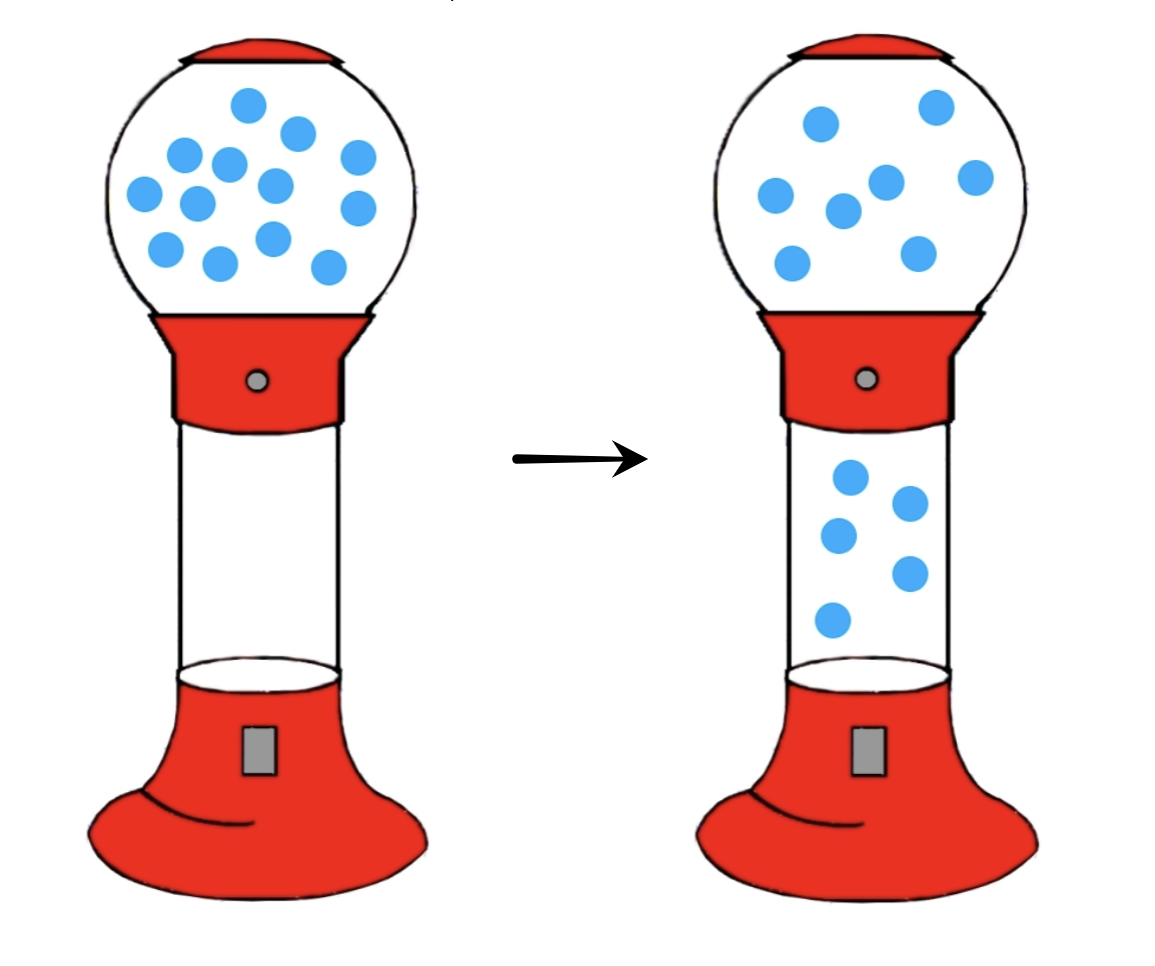
\includegraphics[width=.6\columnwidth]{./img/gumballs2.png}}
\caption{Example display from gumball paradigm. Left: initial display. Right: display with 5 gumballs dropped.  \label{fig:gumball-paradigm}}
\end{figure}

 \begin{table*}[]
 \centering
    \small
    \begin{tabular}{cclll}
    \cline{1-2}
    \toprule
    \textbf{\emph{all}-QUD} & \textbf{\emph{any}-QUD} &  &  &  \\
    \midrule
    \multicolumn{2}{c}{\begin{tabular}[c]{@{}c@{}}You are at a candy store and are testing a row of gumball machines. These are special \\ gumball machines that say how many gumballs you got. However, this report is \\ sometimes faulty.\end{tabular}} &  &  &  \\
    \midrule
    \begin{tabular}[c]{@{}c@{}}The store worker tells you that his boss has threatened \\ to fire him if the gumball machines are left empty, and he \\ really needs this job. He cannot see the machines from \\ the register, but he can normally tell how full they \\ are by the machines' statements.\end{tabular} & \begin{tabular}[c]{@{}c@{}}The store worker tells you that machines sometimes \\ jam and don't deliver any gumballs. His boss has \\ threatened to fire him if the gumball machines stay \\ jammed, and he really needs this job. He cannot see \\ the machines from the register, but he can normally \\ tell if they are working by the machines' statements.\end{tabular} &  &  &  \\
    \midrule
    \begin{tabular}[c]{@{}c@{}}He asks you to tell him if the statement is right or wrong, \\ so that he will know if a machine is empty and needs to be \\ refilled.\end{tabular} & \begin{tabular}[c]{@{}c@{}}He asks you to tell him if the statement is right or wrong, \\ so that he will know if a machine isn't working and need to \\ be fixed.\end{tabular} &  &  &  \\
    \midrule
    \multicolumn{2}{c}{After you hear the statement, you have 4 seconds to notify the store worker, so please make a decision as quickly as possible.} &  &  & 
    \end{tabular}
     \normalsize
    \caption{Cover stories for each QUD condition.\label{tab:coverstories}}
    \end{table*}
  
    
In studies that use truth-value judgment tasks to probe scalar inferences, participants typically complete multiple critical trials of the kind described above \cite{NoveckPosada2003,BottNoveck2004,DegenTanenhaus2015,JasbiEtAl2019}. Participants don't always respond consistently across critical trials \cite<see>[for a detailed response consistency analysis]{DegenTanenhaus2015}, which has led researchers to categorize participants as either ``pragmatic'' or ``literal'' responders and conduct responder type analyses to investigate whether participants' varying response strategies result in varying processing strategies. For instance, \citeNP{DegenTanenhaus2016} found that pragmatic responders were more strongly affected by the experimental manipulation of number term presence than literal responders, who tended to wait for disambiguating information before fixating on target regions of the display. We include such post hoc responder type analyses in our response time analyses. Specifically, we treat responder type as an additional variable that may influence processing times by providing latent contextual support for one over another interpretation: if being a pragmatic responder increases the latent contextual support for the pragmatic response, these responses should be faster than literal responses; conversely for literal responders. 
  
Within each experiment, we followed \citeNP{Degen2013} in manipulating contextual support for the inference via an experiment-level implicit QUD invoked by a cover story that either made the stronger alternative more relevant (\textit{all}-QUD condition, more support for scalar inference) or less relevant (\textit{any}-QUD condition, less support for scalar inference). 


%Participants were assigned to one of the two conditions (\textit{all}-QUD, \textit{any}-QUD) which differed in the cover story they were presented with at the beginning of the experiment (see Table \ref{tab:coverstories}). 
%These cover stories were designed to establish the following implicit QUDs:
%\begin{itemize}
%\item \textbf{\textit{all}-QUD:} Is the machine empty? $\rightarrow$ Did I get all of the gumballs? (\textit{more supportive of scalar inference})
%\item \textbf{\textit{any}-QUD:} Is the machine jammed? $\rightarrow$ Did I get any of the gumballs? (\textit{less supportive of scalar inference})
%\end{itemize}

% \textbf{\textit{all}-QUD} Participants assigned to the \textit{all}-QUD condition read a cover story explaining that they are at a candy store helping the store worker test a row of special gumball machines. These gumball machines report how many gumballs they distribute but are sometimes incorrect in their report. Participants were also told that the store worker's boss has threatened to fire him if the gumaball machines are left empty and he cannot see the machines from the register and can only tell how full they are by their statements. Participants were asked to help the store worker by telling him if this statement is right or wrong by pressing the yes or no key. They were also told that they had 4 seconds to notify the store worker and they should make a decision as quickly as possible. 

% \textbf{\textit{any}-QUD} Participants in the \textit{any}-QUD condition read the same cover story except in their story, the gumball machines sometimes jam and don't deliver gumballs. The store worker's boss has threatened to fire him if the gumball machines stay jammed.


  % \begin{table*}[]
  %   \begin{tabular}{cclll}
  %   \cline{1-2}
  %   \toprule
  %   \textbf{all-QUD} & \textbf{any-QUD} &  &  &  \\
  %   \midrule
  %   \multicolumn{2}{c}{\begin{tabular}[c]{@{}c@{}}You are at a candy store and are testing a row of gumball machines. These are special \\ gumball machines that say how many gumballs you got. However, this report is \\ sometimes faulty.\end{tabular}} &  &  &  \\
  %   \midrule
  %   \begin{tabular}[c]{@{}c@{}}The store worker tells you that his boss has threatened \\ to fire him if the gumball machines are left empty, and he \\ really needs this job. He cannot see the machines from \\ the register, but he can normally tell how full they \\ are by the machines' statements.\end{tabular} & \begin{tabular}[c]{@{}c@{}}The store worker tells you that machines sometimes \\ jam and don't deliver any gumballs. His boss has \\ threatened to fire him if the gumball machines stay \\ jammed, and he really needs this job. He cannot see \\ the machines from the register, but he can normally \\ tell if they are working by the machines' statements.\end{tabular} &  &  &  \\
  %   \midrule
  %   \begin{tabular}[c]{@{}c@{}}He asks you to tell him if the statement is right or wrong, \\ so that he will know if a machine is empty and needs to be refilled.\end{tabular} & \begin{tabular}[c]{@{}c@{}}He asks you to tell him if the statement is right or wrong, \\ so that he will know if a machine isn't working and need to be fixed.\end{tabular} &  &  &  \\
  %   \midrule
  %   \multicolumn{2}{c}{After you hear the statement, you have 4 seconds to notify the store worker, so please make a decision as quickly as possible.} &  &  & \\
  %   \end{tabular}
  %   \caption{Cover stories for each QUD condition.\label{tab:coverstories}}
  %   \end{table*}


\section{Experiment 1: Partitive sentences}

In Exp.~1 we tested whether the QUD  modulates the probability of a scalar inference and whether the QUD and participants' responder type jointly modulate the speed with which pragmatic and literal interpretations are processed. Sentences on critical trials included \emph{some} in its partitive form, which has previously been shown to support the inference \cite{Degen2015}.

Procedure, materials, analyses and exclusions were pre-registered at https://osf.io/49uqm.


\subsection{Methods}

\noindent \textbf{Participants.} We recruited 800 participants on Amazon's Mechanical Turk. Participants were required to have a US-based IP address and a minimal approval rating of 95\%. %They were paid \$2.30 (approximately \$14/hr). 

\noindent \textbf{Materials and procedure.} On each trial, participants saw a display of a gumball machine with 13 gumballs in the upper chamber and an empty lower chamber. After 4 seconds, some number of gumballs moved to the lower chamber (Fig.~\ref{fig:gumball-paradigm}) and a voice reported how many gumballs were distributed. Participants' task was to indicate whether they `agree' or `disagree' with the statement by pressing the F or J key as quickly as possible. The pre-recorded statement was of the form \emph{You got X gumballs}, where X was a quantifier (\textit{some of the},  \textit{all of the}, \textit{none of the}, or a number between 1 and 13). The quantifier and the number of gumballs that dropped to the lower chamber varied.
  
Before proceeding to the main body of the experiment, participants read a cover story to induce an implicit QUD (see Table \ref{tab:coverstories} for cover stories). They completed a scripted demonstration that introduced a gumball store worker who will be fired if he either fails to re-fill a gumball machine when it's empty (\emph{all}-QUD condition) or if he fails to fix a machine if it's not dispensing gumballs (\emph{any}-QUD condition). To ensure that participants paid attention to the cover story, they were asked a multiple-choice question about the condition under which the store worker will be fired. If participants answered this question incorrectly, they were presented with the cover story again and repeated the demonstration. Halfway through the experiment, participants were asked to answer the multiple-choice question again. This was done to prevent the decay of the implicit QUD over time.  
 

There were 4 practice trials with \textit{all} and \textit{none}. On half of these trials, the statements were correct and on the other half they were incorrect. After the practice trials, participants completed 72 experimental trials (see Table \ref{tab:stimuli}). On 32   trials, the expected answer was `agree', on another 32 trials, the expected answer was `disagree'. The remaining 8 trials were  critical trials on which all 13 gumballs dropped to the lower chamber and participants heard the partitive scalar statement \emph{You got some of the gumballs}. To reiterate, if participants pressed J to agree with the statement, they interpreted it literally; if they pressed F to disagree, they interpreted it pragmatically.


  \begin{table}
      \begin{tabular}{lccccccc}
      \midrule
      \multicolumn{8}{c}{\textbf{Set size}} \\
      \textbf{Quantifier} & 0 & 2 & 5 & 8 & 11 & 13 & \multicolumn{1}{l}{\textbf{Total}} \\
      \midrule
      \textit{some of/some} & 4 & 1 & 1 & 1 & 1 & 8 & 16 \\
      \textit{all of} & 2 & 1 & 2 & 1 & 2 & 8 & 16 \\
      \textit{none of} & 4 & 1 & 0 & 1 & 1 & 1 & 8 \\
      number & 3 & 7 & 7 & 7 & 5 & 3 & 32 \\
      \bottomrule
      \textbf{Total} & 13 & 10 & 10 & 10 & 9 & 20 & 72
      \end{tabular}
    \caption{Distribution of experimental trials over quantifiers and set sizes. \label{tab:stimuli}}
  \end{table}
  
  
\noindent \textbf{Exclusions.} We excluded participants who were self-reported non-native English speakers (n=20), participants who incorrectly answered the second comprehension question more than twice (n=17) and participants with accuracy lower than 85\% on non-critical trials (n=235). Only responses to critical trials are reported below. These exclusions had no qualitative effect on the results discussed below.

%\noindent \textbf{Analysis and predictions} Only responses on critical trials were  analyzed here and in Exp.~2. We conducted three types of analyses to address the two questions of interest. 
%\begin{enumerate}
%\item Does the QUD modulate the probability of drawing a scalar inference?
%\item Does the contextual support that an interpretation (either pragmatic or literal) receives
%\end{enumerate} 
% To this end, we conducted a mixed effect logistic regression predicting the log odds of pragmatic ``no'' over literal ``yes'' responses. 
 
 
\noindent \textbf{Analysis.}  Only responses on critical trials were  analyzed here and in Exp.~2. We conducted three types of analyses to address the questions of interest. First, we analyzed judgments to test whether the contextual QUD modulated scalar inferences. To this end, we conducted mixed effects logistic regression predicting the log odds of a pragmatic over a literal response from a fixed effect of QUD and the maximal random effects structure justified by the design --  random by-participant intercepts. Second, we analyzed participants' response consistency and categorized them as  literal or pragmatic responders. Third, we tested the prediction made by the constraint-based account  that responses that reflect a particular interpretation (pragmatic or literal) should be processed more quickly, the greater the contextual support for the interpretation. To this end, we conducted a mixed effects linear regression model predicting log-transformed response time from fixed effects of QUD, response type, and responder type, with the maximal random effects structure justified by the design -- random by-participant intercepts and slopes for response type. All fixed effect predictors were centered before entering their respective analysis.
 
 
\subsection{Results and discussion}


\noindent \textbf{Judgments.} Proportion of pragmatic responses on critical trials are shown on the left in Figure~\ref{fig:judgments}. We observed a main effect of QUD such that there were more pragmatic responses in the \textit{all}-QUD condition (78\%) compared to the \textit{any}-QUD condition (70\%, $\beta$=1.27, SE=0.53, p$<$.05), replicating previous QUD effects on scalar inference \cite{DegenGoodman2014,Zondervan2010}. 


\begin{figure}
\centering
  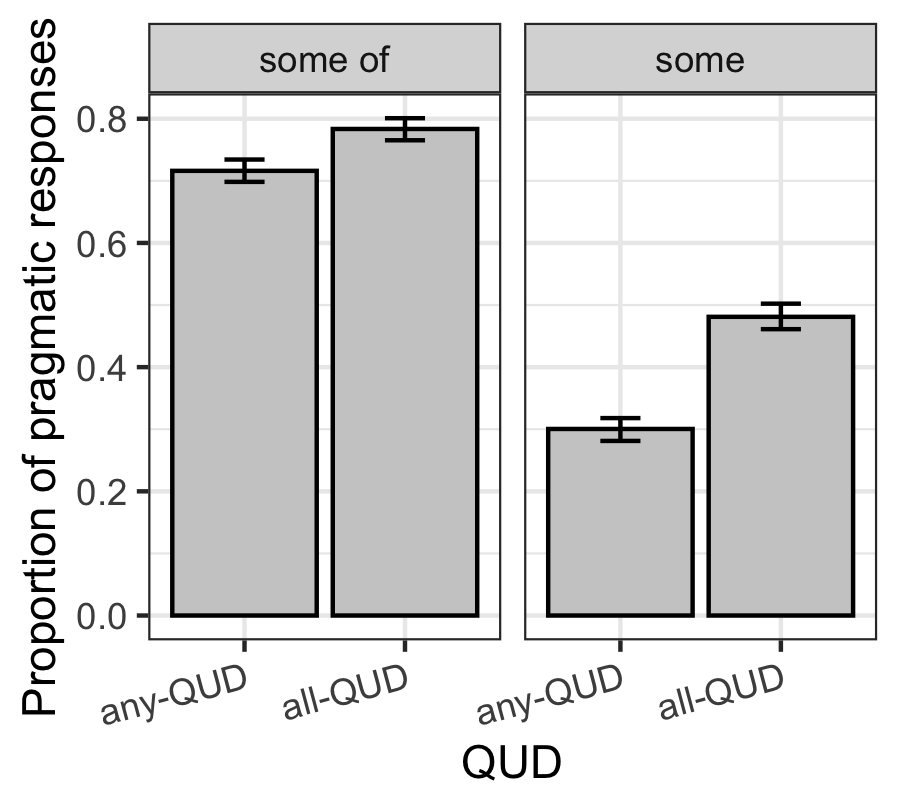
\includegraphics[width=.75\columnwidth]{plots/judgements.png}
  \caption{Proportion of pragmatic responses on partitive \emph{some of} (Exp.~1, left) and non-partitive \emph{some} (right, Exp.~2) critical trials. Error bars indicate bootstrapped 95\% confidence intervals. \label{fig:judgments}}
  \end{figure}

\noindent \textbf{Analysis of variability in judgments.} The top panel of \figref{fig:proportion} shows the distribution of participants over number of pragmatic responses given on critical trials. Participants who either gave 0 or 8 pragmatic responses were completely consistent in their responses (60\%, of which 19\% completely literal and 81\% completely pragmatic). \figref{fig:proportion} reflects \figref{fig:judgments} and shows that the distribution of pragmatic responses in the \emph{all}-QUD condition is shifted towards the more pragmatic end of the continuum compared to the \emph{any}-QUD condition. Thus, while some participants were entirely consistent, there was also substantial inter-participant variability in consistency. For the purpose of the subsequent response time analyses, and following previous researchers \cite{BottNoveck2004,DegenTanenhaus2015}, we divided participants into two groups:  participants with more than 4 pragmatic responses were categorized as \emph{pragmatic} responders (73\%) and participants with fewer than 4 pragmatic responses were categorized as \emph{literal} responders (23\%). 18 participants (3\%) gave an equal number of pragmatic and literal responses and were excluded from the response time analysis.


\begin{figure}
  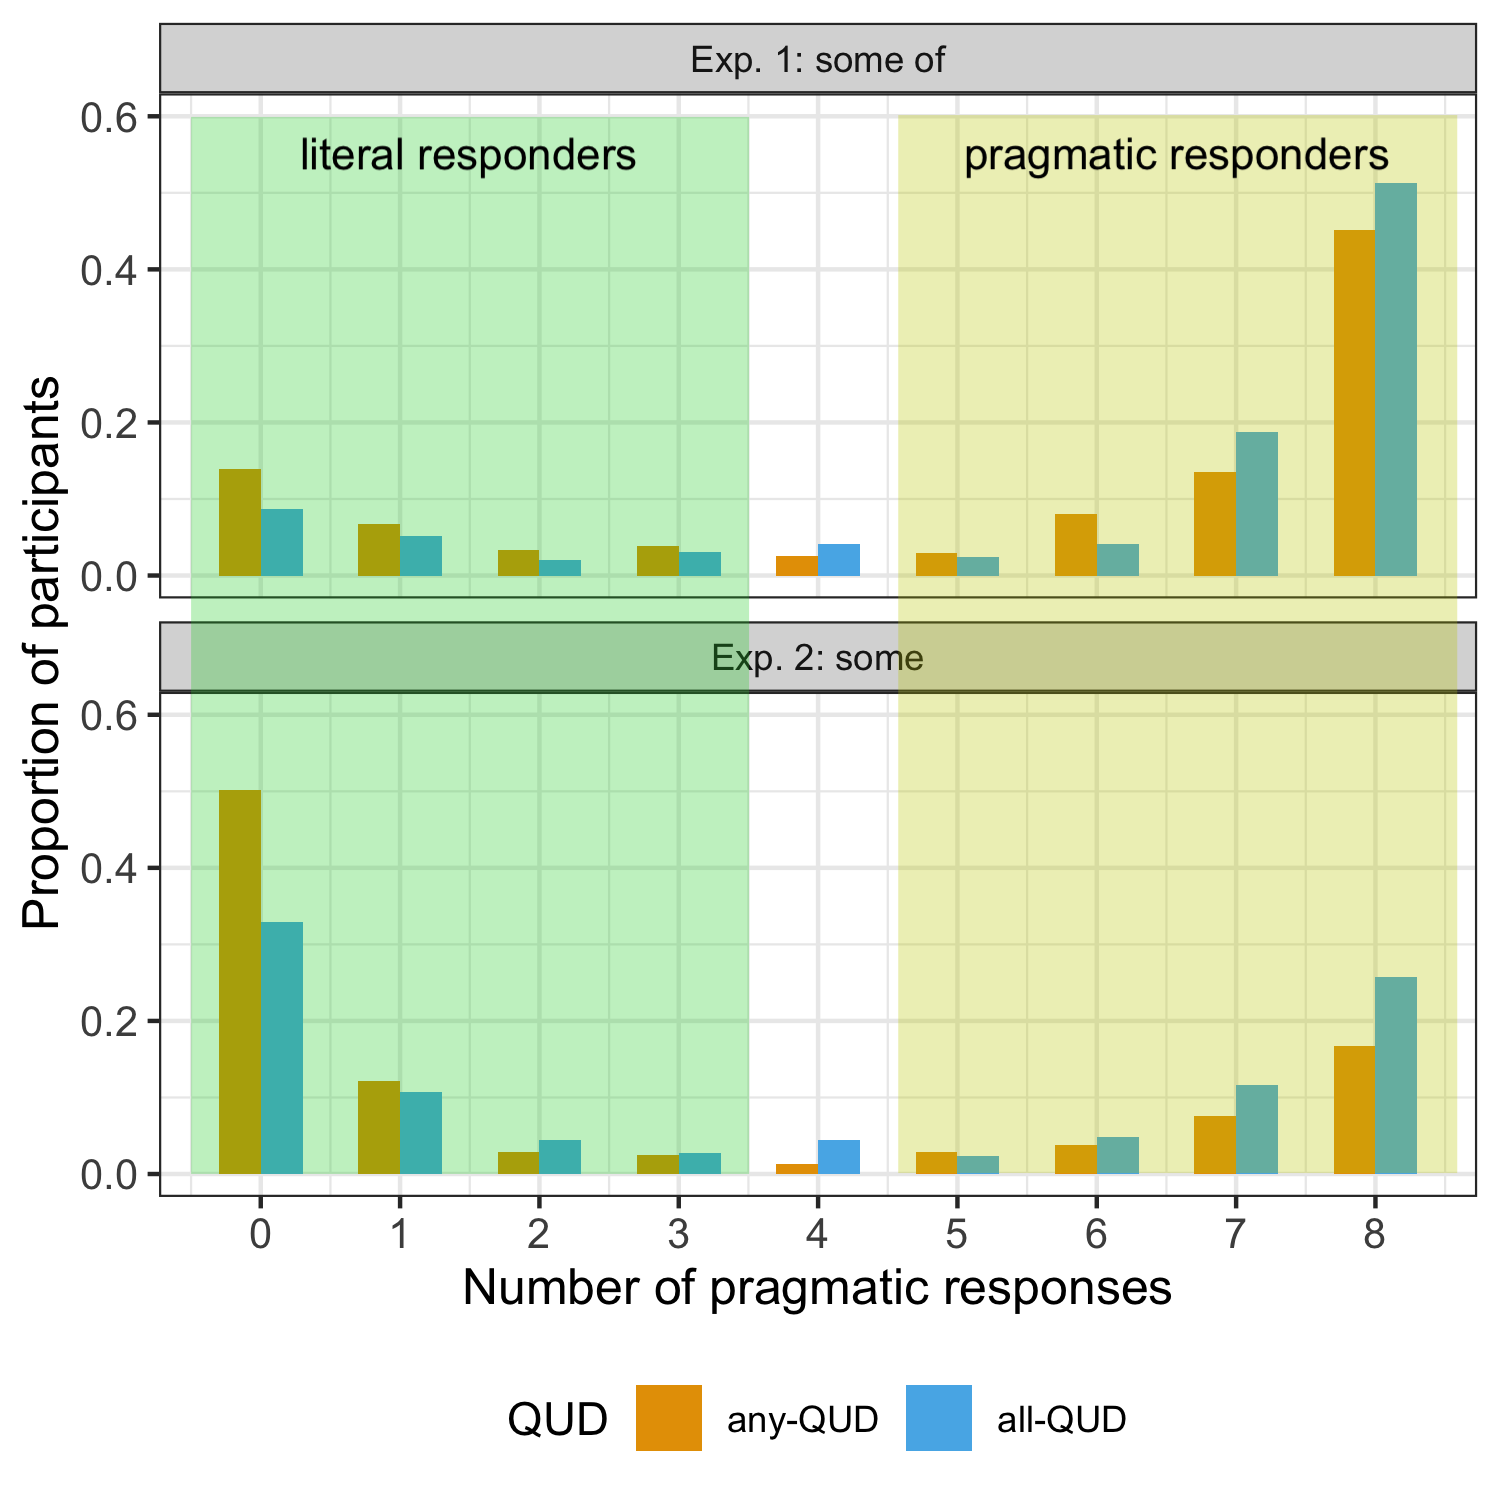
\includegraphics[width=\linewidth]{plots/proportion.png}
  \caption{Distribution of participants over number of pragmatic responses given on critical trials. Participants with $< 4$ pragmatic responses were categorized as literal responders (green), participants with $> 4$ responses as pragmatic responders (yellow). }
  \label{fig:proportion}
\end{figure}

  
\noindent \textbf{Response times.} Response times are shown in the top panels of \figref{fig:responsetimes}. We observed an interaction between QUD and response ($\beta$=-8.16, $SE$=3.40, $t$=-2.40, $p$$<$.05). Simple effects analysis revealed that this interaction was driven by pragmatic responses being slower than literal responses under the \textit{any}-QUD ($\beta$=6.70, SE=3.38, t=1.98, p$<$.05), while there was no difference in response times under the \textit{all}-QUD ($\beta$=-1.44, SE=3.59, t=3.75, p$<$.69). We also observed an interaction between responder type and response ($\beta$=-2.37, SE=3.25, t=-7.29, p$<$.0001). 
Simple effects analysis revealed that this interaction was driven by pragmatic responses being faster than literal responses for \emph{pragmatic}  responders ($\beta$=-1.69, SE=3.07, t=-5.53, p$<$.0001) and pragmatic responses being slower than literal responses for \emph{literal} responders ($\beta$=6.70, SE=3.38, t=1.98, p$<$.05). 

These results provide evidence against the costly inference account: rather than pragmatic responses being generally slower than literal responses, they were only so when given by literal responders or when given in response to the \emph{any}-QUD, which was found to provide less contextual support for the inference than the \emph{all}-QUD. Moreover, these results also excitingly show that pragmatic responses can even be faster than literal responses under certain conditions, namely when produced by pragmatic responders. These results are consistent with the constraint-based account. To test whether the contextual effects remain stable when overall decreasing the contextual support for the inference, we conducted Exp.~2.


\section{Experiment 2: Non-partitive sentences}

Exp.~2 was identical to Exp.~1, with the exception that the sentence on critical trials was the non-partitive \emph{You got some gumballs}, previously shown to yield lower inference rates than its partitive counterpart. %we tested whether the absence of the partitive, previously shown to decrease the contextual support for the inference, would decrease the scalar inference rate. We also investigated whether the QUD and responder type effects observed in Exp.~1 would replicate without the contextual support of the lexical cue.

\subsection{Methods}

\noindent \textbf{Participants.} We recruited 800 participants on MTurk. %Amazon's Mechanical Turk. %Participants were required to have a US-based IP address and a minimal approval rating of 95\%, and they were paid \$2.3 (approximately \$14/hr).

\noindent \textbf{Materials and procedure.} The materials and procedure were identical to Exp.~1 except on critical trials, where participants heard the non-partitive statement \emph{You got some gumballs}.

\noindent \textbf{Exclusions.} As in Exp.~1, we excluded non-native English speakers (n=19), participants who got the second comprehension question wrong more than twice (n=29), and participants that had accuracy lower than 85\% on non-critical trials (n=217).


\begin{figure}
\centering
  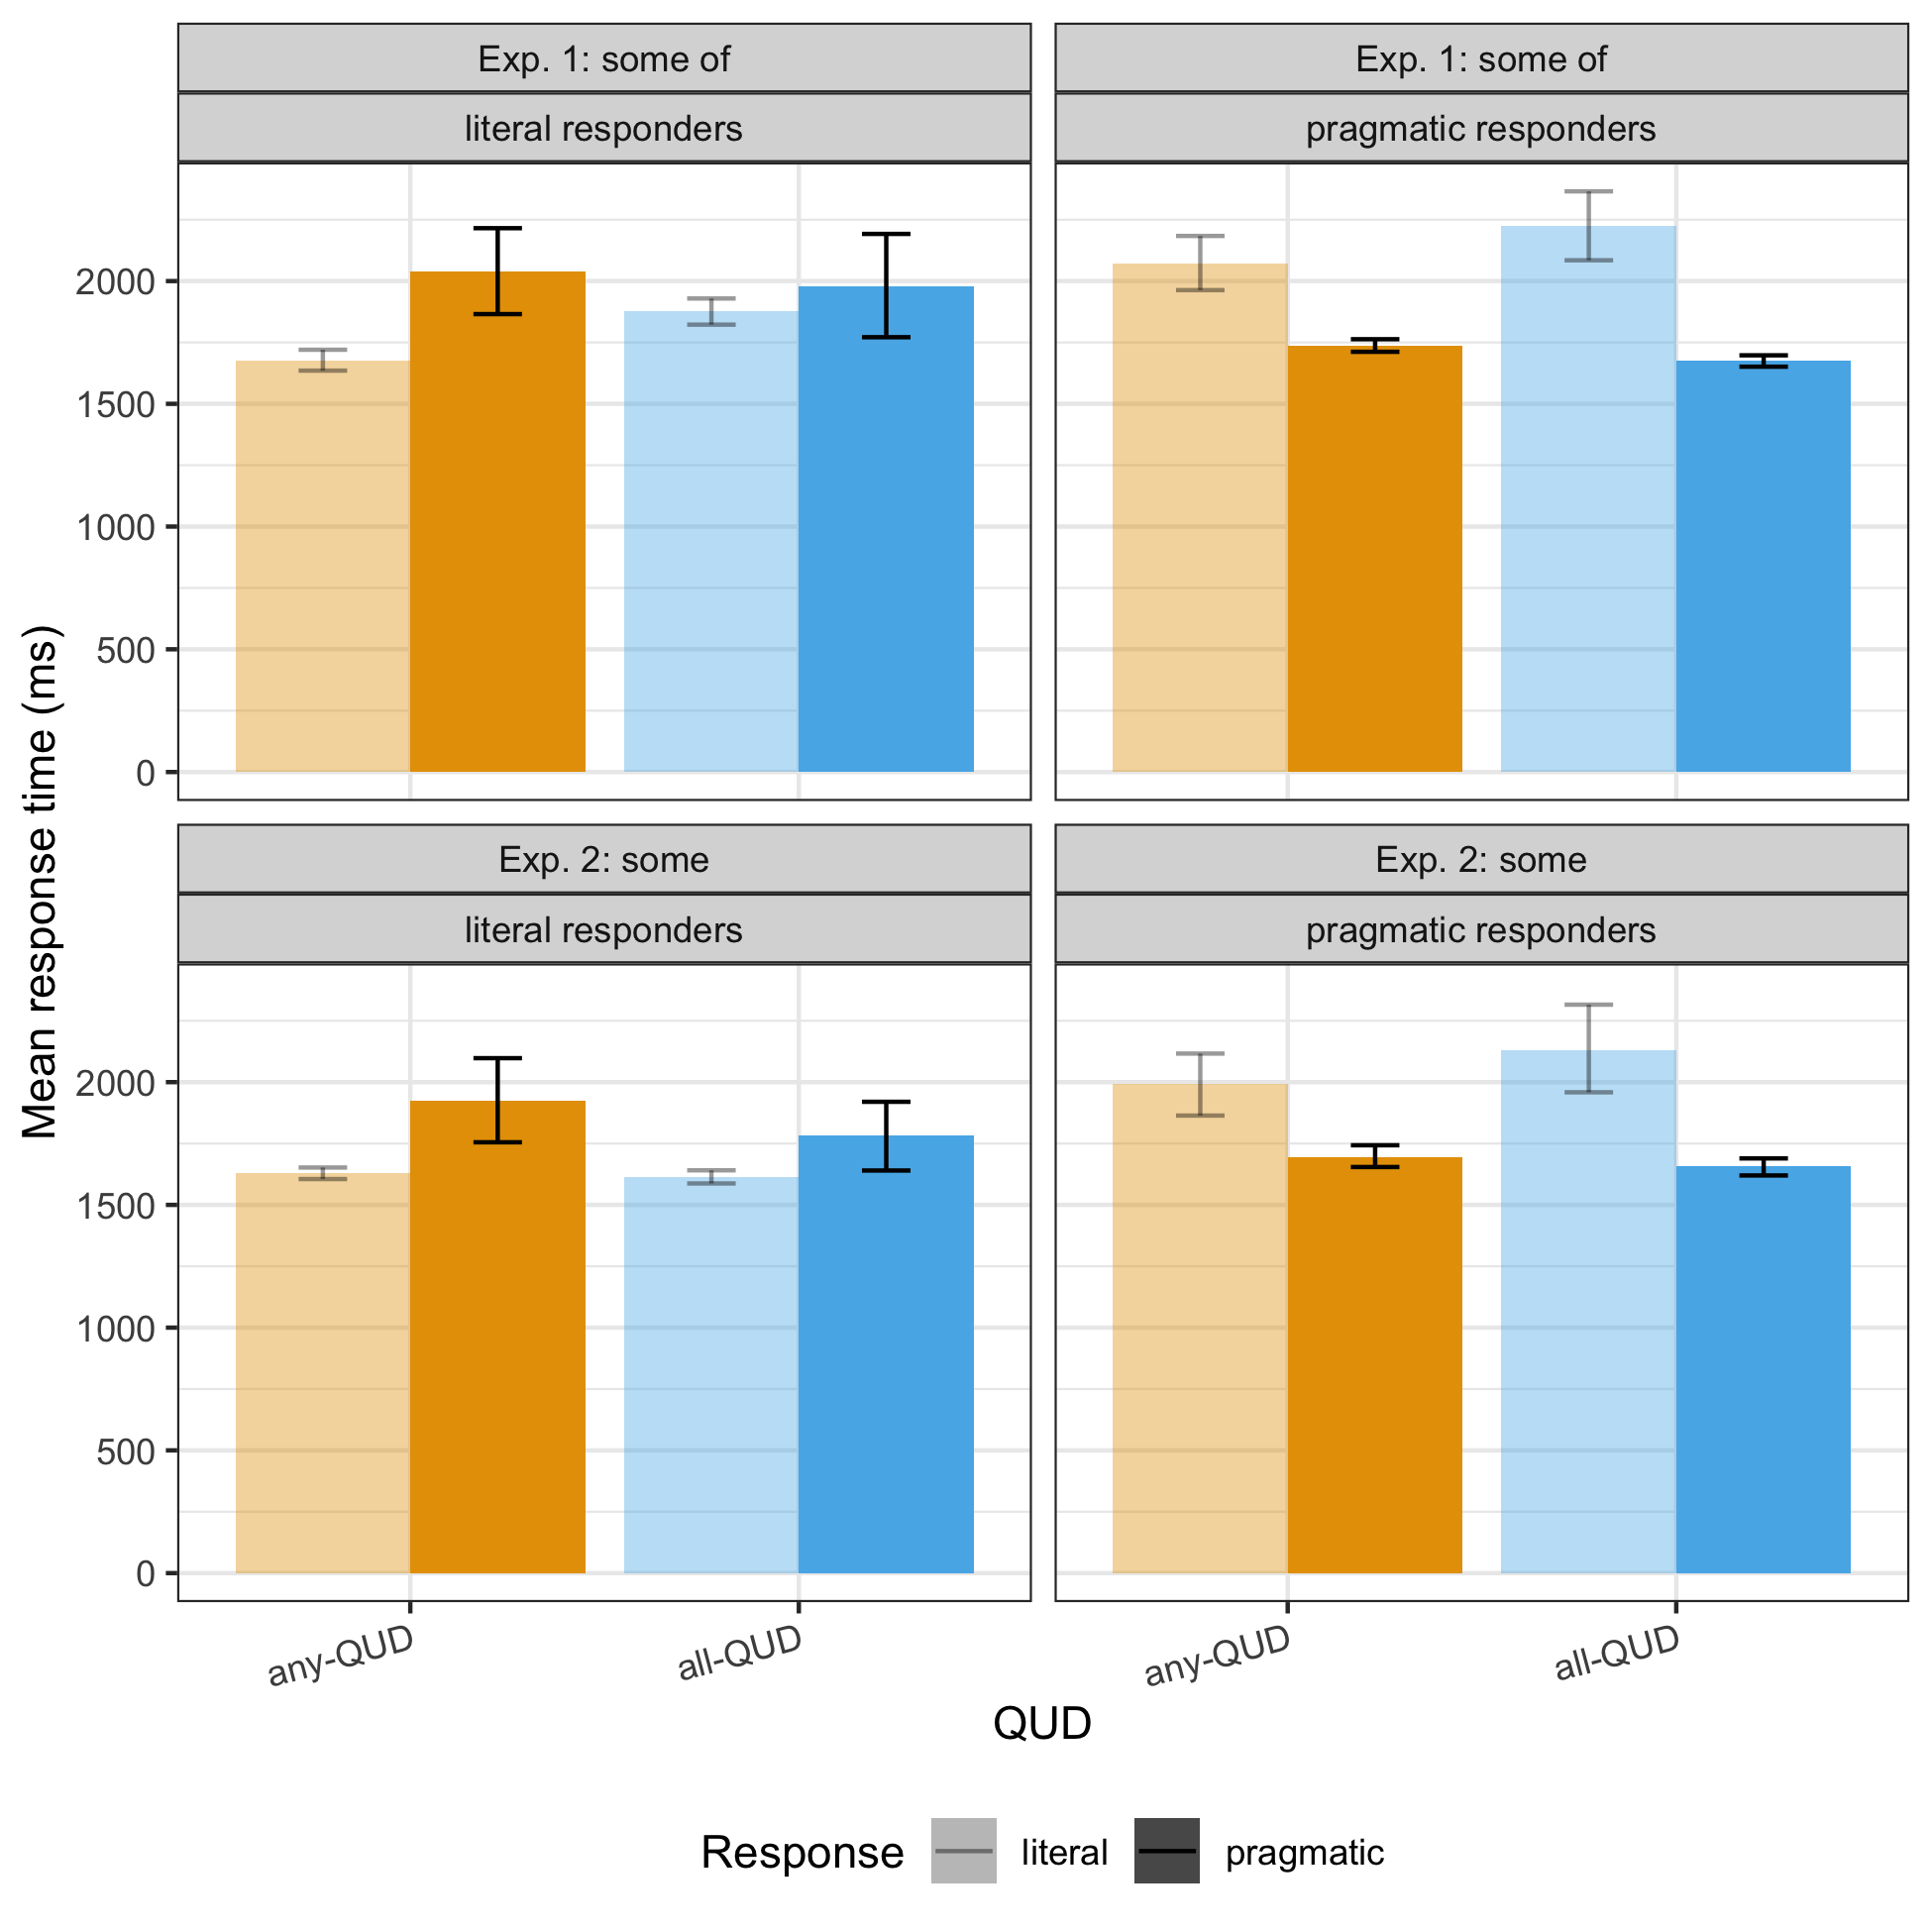
\includegraphics[width=\columnwidth]{plots/responsetimes}
  \caption{Mean response times for literal (light) and pragmatic (dark) responses generated by literal (left column) and pragmatic (right column) responders on partitive \emph{some of} (Exp.~1, top panels) and non-partitive \emph{some} (Exp.~2, bottom panels) critical trials. }
  \label{fig:responsetimes}
\end{figure}

\subsection{Results}

\noindent \textbf{Judgments.} Proportion of pragmatic responses on critical trials are shown on the right in Figure~\ref{fig:judgments}. We replicated the QUD effect found in Exp.~1: participants in the \textit{all}-QUD condition gave more pragmatic "disagree" responses (48\%) than participants in the \textit{any}-QUD condition (30\%, $\beta$=3.07, SE=0.63, p$<$.0001). However, as is evident from \figref{fig:proportion}, the rate of pragmatic responses was greatly reduced overall compared to Exp.~1. This was borne out in a mixed effects logistic regression where the data from both experiments was  pooled and sentence form added as a fixed effect predictor ($\beta$=5.89, SE=0.55, p$<$.0001), replicating previous studies \cite{DegenTanenhaus2015,Degen2015}. 


\noindent \textbf{Analysis of variability in judgments.} The bottom panel of \figref{fig:proportion} shows the distribution of participants over number of pragmatic responses given on critical trials. Reflecting the average changes in  Fig~\ref{fig:proportion}, overall and in the \emph{any}-QUD condition, the distribution of  responses shifted towards the more literal end of the continuum compared to Exp.~1 and the \emph{all}-QUD condition.  22\% of participants were completely consistent in providing pragmatic responses compared to 40\% of participants who consistently responded literally. Overall, 38\% of participants were categorized as pragmatic responders and 58\% as literal responders. 16 participants (3\%) were excluded from the response time analysis because they gave equal number of pragmatic and literal responses.

\noindent \textbf{Response times.} \lk{these effects are not significant anymore} Response times are shown in the bottom panels of \figref{fig:responsetimes}. We closely replicated the results from Exp.~1, both qualitatiively and quantiatively. In particular, we observed an interaction between QUD and response ($\beta$=-0.07, $SE$=0.03, $t$=-2.14, $p$$<$.05). Simple effects analysis revealed that this interaction was driven by pragmatic responses being slower than literal responses under the \textit{any}-QUD ($\beta$=0.08, SE=0.03, t=2.75, p$<$.007), while there was no difference in response times under the \textit{all}-QUD ($\beta$=0.03, SE=0.03, t=1.12, p$<$.27). We also observed an interaction between responder type and response ($\beta$=-0.27, SE=0.03, t=-8.38, p$<$.0001). Simple effects analysis revealed that this interaction was driven by pragmatic responses being faster than literal responses for \emph{pragmatic}  responders ($\beta$=-0.16, SE=0.03, t=-4.91, p$<$.0001) and pragmatic responses being slower than literal responses for \emph{literal} responders ($\beta$=0.09, SE=0.03, t=2.75, p$<$.007). 

It would have been interesting to assess the effect of the partitive form on response times across the two experiments -- if the strong version of the constraint-based is right, the partitive should lead to faster pragmatic responses than the non-partitive form. Unfortunately, directly comparing the response time results from Exps.~1 and 2 is not  possible because of the different overall lengths of the audio files, which is reflected in the response times (partitive utterances were on average 132ms longer than non-partitive ones).

\begin{figure}
  \centering
    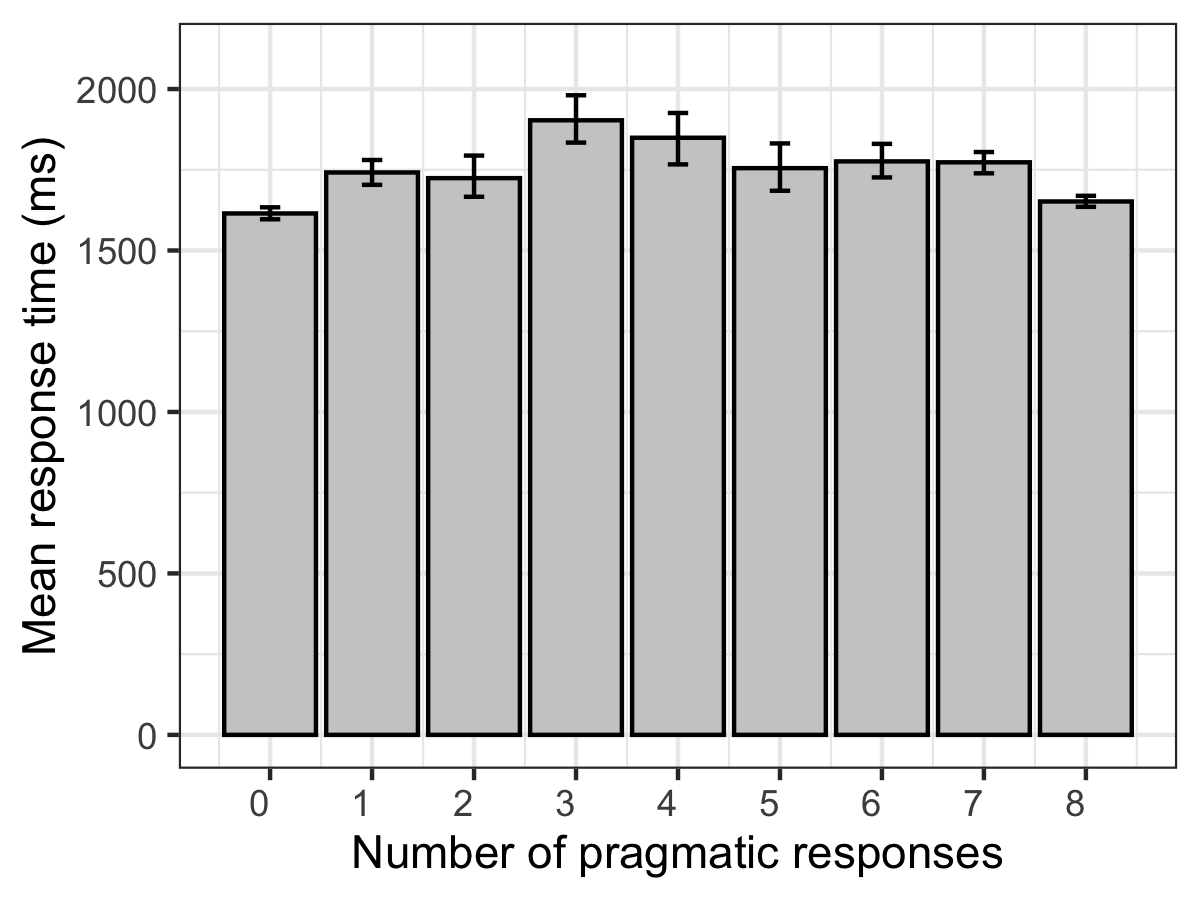
\includegraphics[width=\columnwidth]{plots/consistency}
    \caption{\lk{new plot} Response time as a function of response consistency.}
    \label{fig:consistency}
  \end{figure}

%In order to compare the response times of participants from Exp.~1 and 2, we had to calculate each response time with respect to the length of the audio stimuli participants heard. For each experiment, we subtracted the length of the onset of the word "gumball" (Exp.~1: 868ms, Exp.~2: 736ms) from all response times. This ensured that response times \lk{XXX}. We were interested in whether the lack of the partitive would slow down pragmatic responses and speed up literal responses compared to its partitive counterpart. We analyzed the data using a mixed effects linear regression model with by-participant intercepts to predict log-transformed response times. The model included centered fixed effects of quantifier and response. We found a significant interaction between quantifier and response such that ($\beta$=-0.10, SE=0.04, t=2.48 p$<$.05) \lk{explain}

%\lk{We weren't able to replicate the QUD effect on the speed of scalar inferences when the non-partitive form was used.} \jd{when i run the analyses everything comes out the same as in exp 1}

%\lk{which one do we want to focus on?}
%Finally, we ran a full model on the pooled data with QUD, quantifier, response and responder type as centered predictors. We found a main effect of quantifier ($\beta$=5.24, SE=1.52, t=3.45, p$<$.001), response ($\beta$=-8.69, SE=1.15, t=-7.58, p$<$.001), an interaction between qud and response ($\beta$=-1.06, SE=2.29, t=-4.62, p$<$.001), and an interaction between response and responder type ($\beta$=-2.69, SE=2.30 t=-11.68, p$<$.001)

% We also ran a full model on the pooled data and predicted log-transformed response times from centered fixed effects of QUD, quantifier, response and responder type. The model included by-participant intercepts. We found a main effect of partitive ($\beta$=5.24, SE=1.52, t=3.45, p$<$.001), an interaction between qud and response ($\beta$=-1.06, SE=2.29, t=-4.62, p$<$.001), and an interaction between response and responder type ($\beta$=-2.69, SE=2.30 t=-11.68, p$<$.001).


\section{General discussion and conclusion}

The issue of whether or not scalar inferences generally incur a processing cost has been the subject of much debate. Here we have added an additional data point against costly inference accounts: we have identified contextual conditions under which pragmatic responses are provided more quickly than literal responses, to our knowledge the first time the reversal of this classic response time pattern has been shown. We have also replicated previous findings showing that both a QUD that makes the stronger alternative more contextually relevant sand the presence of the partitive increase the rate of scalar inferences. Under the strong constraint-based prediction, response times associated with the literal and pragmatic interpretation should have been directly related to the amount of contextual support they received. Instead, rather than finding a decrease/increase in response times for pragmatic responses under the \emph{all/any}-QUD compared to literal responses, respectively, we observed the predicted difference in pragmatic and literal response times only in the \emph{any}-QUD condition. However, the strongest effect on response times was the interaction between responder type and response. That pragmatic responders generally provided faster pragmatic than literal responses and vice versa for literal responders suggests that, rather than directly affecting response times, contextual cues to pragmatic meaning may guide listeners' overall expectations for likely meanings, which in turn affect how much processing effort -- and consequently, response time -- must be invested to arrive at a particular response. We thus interpret these results as further limited evidence for constraint-based accounts of pragmatic processing. The complex causal links between contextual cues to meaning and inferential processing effort require further investigation, but it is clear from this and previous work that treating scalar inferences as monoliths with a particular associated inferential effort is unlikely to yield a satisfying theory of pragmatic processing.


%\begin{figure}
%  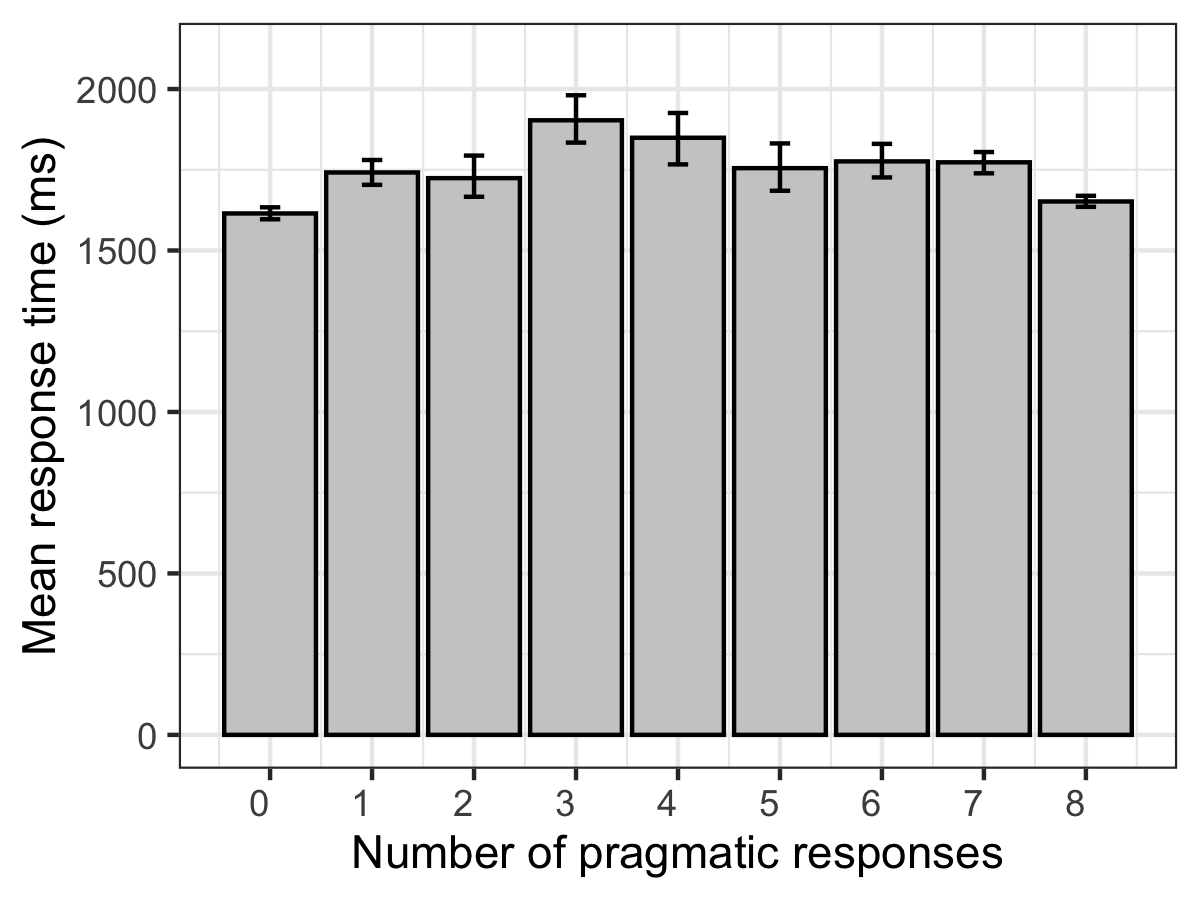
\includegraphics[width=\columnwidth]{plots/consistency.png}
%  \caption{Mean response times for participants grouped based on the number of pragmatic responses they gave. \label{fig:consistency}}
%\end{figure}

%\section{References Instructions}
%
%Follow the APA Publication Manual for citation format, both within the
%text and in the reference list, with the following exceptions: (a) do
%not cite the page numbers of any book, including chapters in edited
%volumes; (b) use the same format for unpublished references as for
%published ones. Alphabetize references by the surnames of the authors,
%with single author entries preceding multiple author entries. Order
%references by the same authors by the year of publication, with the
%earliest first.
%
%Use a first level section heading, ``{\bf References}'', as shown
%below. Use a hanging indent style, with the first line of the
%reference flush against the left margin and subsequent lines indented
%by 1/8~inch. Below are example references for a conference paper, book
%chapter, journal article, dissertation, book, technical report, and
%edited volume, respectively.


\bibliographystyle{apacite}

\setlength{\bibleftmargin}{.125in}
\setlength{\bibindent}{-\bibleftmargin}

\bibliography{cogsci}

\end{document}
